Durante este capítulo serão descritas em detalhes as diferentes etapas de funcionamento da luva Hand.io e será explicado como os objetivos deste trabalho serão satisfeitos.

\section{Visão geral do método da Hand.io}

A Hand.io é uma luva de controle que permite que quem a use realize gestos para controlar os dispositivos disponíveis em um dado ambiente. O projeto conta com uma luva de pano com um dispositivo preso ao tecido, que lê os movimentos da mão do usuário e uma central de processamento posicionada em um local estratégico, que recebe os sinais dos gestos através de uma conexão sem fio e executa as ações previamente definidas correspondentes a eles.

\begin{figure}[ht]
    \centering
    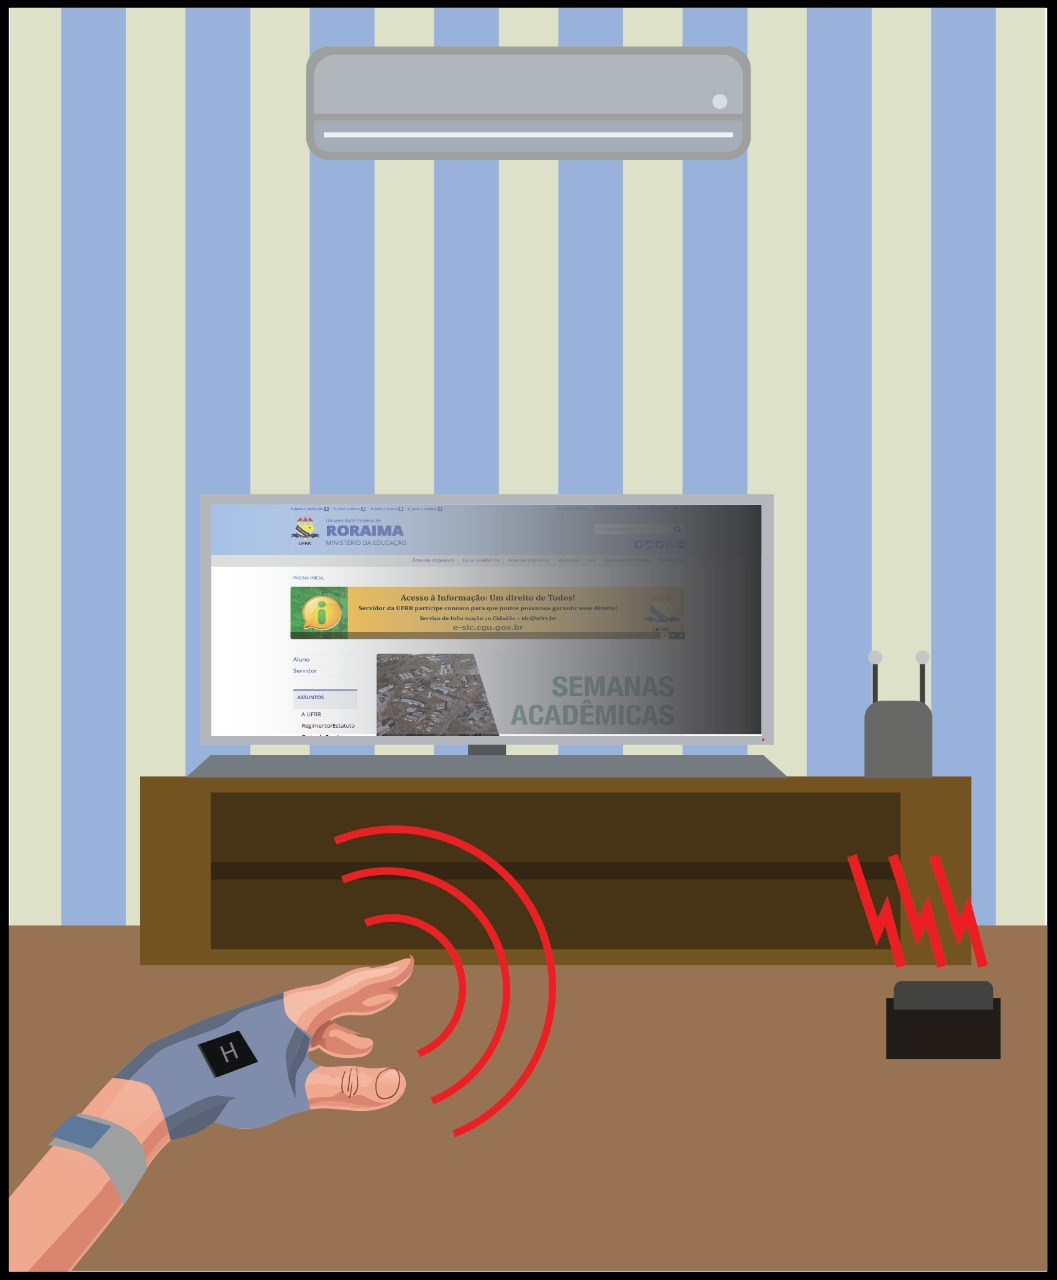
\includegraphics[width=0.5\textwidth, keepaspectratio]{resources/bigpicture.jpeg}
    \caption{Visão geral do protótipo}
    \label{fig:bigpicture}
\end{figure}

Os sinais dos movimentos são processados pela central utilizando algoritmos de aprendizado de máquina, que ajustam os valores de referência dos gestos à cada vez que o usuário os realiza, buscando aumentar a precisão do reconhecimento dos gestos.

%Após os gestos terem sido reconhecidos com sucesso, a central de controle realiza a ação que 

\section{Fluxo de execução da Hand.io}

A figura~\ref{fig:fluxograma}, descreve o método proposto para a luva Hand.io através de um fluxograma, mostrando as diferentes etapas de funcionamento da luva de maneira sequencial.

\begin{figure}[ht]
    \centering
	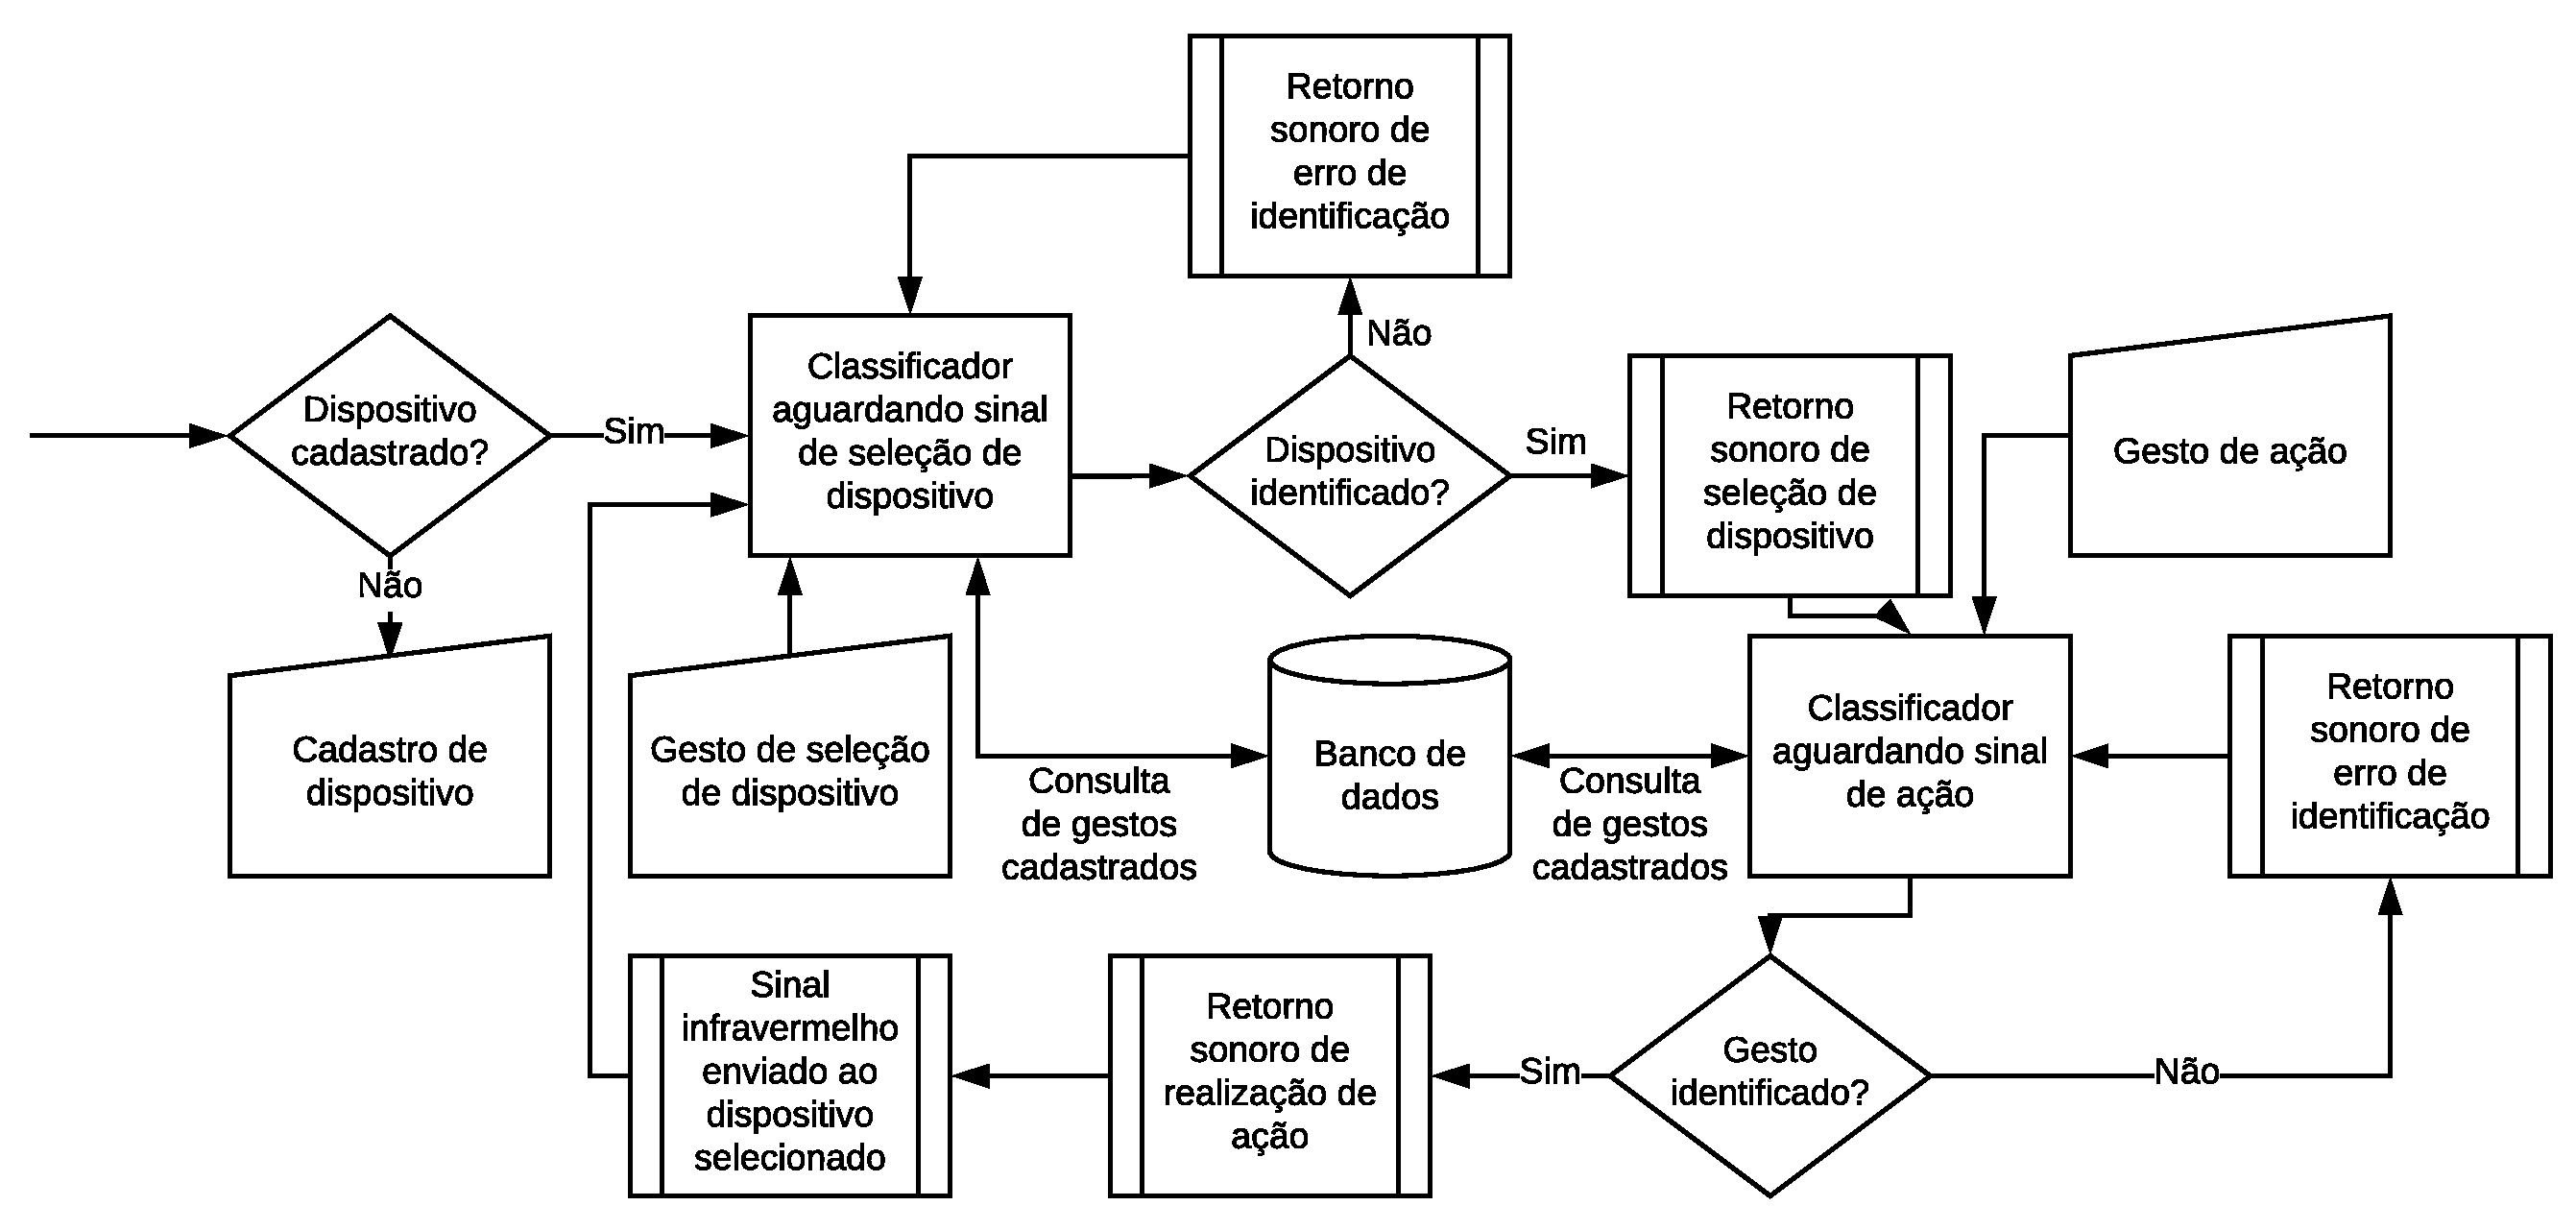
\includegraphics[width=\textwidth, keepaspectratio]{resources/fluxograma.pdf}
	\caption{Fluxograma da Hand.io}
	\label{fig:fluxograma}
\end{figure}

\begin{itemize}
    \item A posição inicial do fluxograma é definida por uma \textbf{seta sem origem} a partir da qual são realizadas as checagens iniciais do sistema.
    \item Os \textbf{losangos} representam condições onde dependendo do resultado o fluxo do sistema pode ser alterado, no primeiro momento é verificada a conexão com a luva de controle e logo depois o sistema verifica se existem dispositivos cadastrados, caso não existam o sistema aguarda pela inserção de dispositivos no banco de dados.
    \item Os \textbf{trapézios} representam ações externas que são realizadas pelo usuário, seja a partir da luva ou a partir do dispositivo que será utilizado para realizar o cadastro de novos dispositivos. 
    \item \textbf{Retângulos} representam processos internos do sistema 
e quadrados com barras laterais representam os processos predefinidos do sistema.
    \item O banco de dados que irá armazenar os dados de gestos e códigos de infra-vermelhos de controle de dispositivos, está representado por um \textbf{cilindro} encontrado na parte central da figura.
\end{itemize}




\section{Captura de Dados Baseado em Movimentos de Amplitude de Punho e Mão}

A ideia principal da luva Hand.io é que o usuário controle seu ambiente utilizando gestos da maneira mais natural possível, para isso os movimentos do usuário são capturados constantemente e enviados para a central de em tempo real até que seja identificado um gesto correspondente a um dispositivo cadastrado, como pode ser observado na figura~\ref{fig:fluxograma}.

A luva Hand.io utilizará dois sensores para realizar a captura dos movimentos da mão do usuário, um acelerômetro e um giroscópio. Estes dois sensores foram escolhidos visando evitar problemas os encontrados no trabalho de \cite{uwave:2009} encontrado na seção \ref{cor:uwave} que sofre problemas de precisão devido a presença de apenas um sensor acelerômetro.

Os sensores 



\subsection{Conexão com a central de processamento}

A conexão entre a luva e a central será realizada utilizando o protocolo de redes sem fio IEEE 802.11  \cite{802.11:1997}, conhecida popularmente como Wi-Fi, através de uma rede LAN. Os dados enviados irão seguir o padrão de codif

\section{Reconhecimento de Padrões Baseado em Movimentos e Ações}



\section{Modelo de Conexão Entre Dispositivos Eletrônicos}

\section{Inferência de Comportamentos para Acionamento de Dispositivos Eletrotônicos}

\section{Modelo de Prototipação}

\begin{figure}[ht]
    \centering
    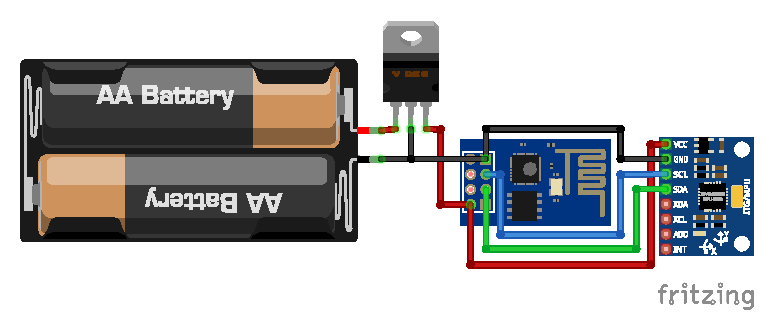
\includegraphics{resources/esquematico_tcc_bb.pdf}
    \caption{Esquemático do protótipo da luva}
    \label{fig:my_label}
\end{figure}

\begin{figure}[ht]
    \centering
    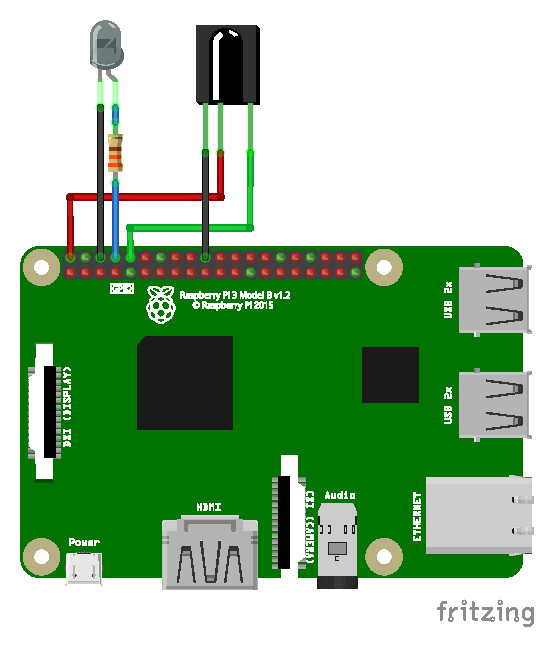
\includegraphics{resources/esquematico_central_bb.pdf}
    \caption{Esquemático da central de processamento de sinais e execução de ações}
    \label{fig:esq_central}
\end{figure}

%\section{Cronograma}